\documentclass[10pt,conference,compsocconf]{IEEEtran}

\usepackage{hyperref}
\usepackage{graphicx}
\usepackage{xcolor}
\usepackage{blindtext, amsmath, comment, subfig, epsfig }
\usepackage{grffile}
\usepackage{caption}
%\usepackage{subcaption}
\usepackage[utf8]{inputenc}


\title{CS-523 SecretStroll Report}
\author{Laval Maxime, Carles Victor}
\date{April 2020}

\begin{document}

\maketitle

\section{Attribute-based credential}

\subsection{Issuance Protocol}

The first step of the Attribute based credential authentication is the issuance of the credentials. To do so, we decided that the user's attributes would be his username, whereas the issuer's attributes would be all the subscriptions the user sends to it. This way, we have the union of both subsets as the whole set of all the user's attributes. As a specification of implementation, we decided to create dictionaries for the user and issuer attributes that map $Y_{i}$ to the corresponding $a_{i}$. All $Y_{i}$ are computed by the server when generating the keys, and they are stored in the public key at the index corresponding to each attribute, the last one being the username. We also stored all the attributes in the public key, as it is easier for some methods to access attribute and retrieve indexes based on the size. 
This way, if a method needs the $Y_{i}$ of a given attribute, it can simply search for the index i of the attribute in the pk and get the value at index i+1 (since g is the first value stored in the pk).
When creating the issue request, following a Fiat-Schemir heurisitc, the user sends a commitment C to the issuer, as well as a challenge c (which is a sha256 hash $H(pk,C,R)$), and a pre-computed response s. Since it is the user that computes the response, the proof is non-interactive, meaning that the issuer doesn't have to do anything except verifying that the challenge he receives was correctly computed, hence proving that the user really has the attributes. Since the issuer doesn't have the user's attributes, it can't compute $C = g^t \prod_{i e U}{Y_{i}^{a_{i}}}$ . 
But, it can compute R'. 
\\	
\hspace{1cm}
R is computed by the user as $g^{rt} \prod_{i e U}{Y_{i}^{ra_{i}}}$, where $rt$ and $ra_{i}$, for i e U, are random values chosen by the user. 
\\	
\hspace{1cm}

$ R' = C^c g^{st} \prod_{i e U}{Y_{i}^{sa_{i}}}$, where $st = rt - c*t$ and $sai = ra_{i} - c*a_{i}$ for i e U. This way, this should all simplify in a way that R' is equal to R, resulting in a same hash a c. The issuer doesn't have to know the user's attributes, it just has to know the indexes to find the corresponding $Y_{i}$ for the responses values $sai$.
If R = R', then the proof is valid, and the user can obtain his credentials. The credentials are all his subscriptions and his username.

\subsection{Showing Protocol}
To prove that the user has the right credentials, we use a similar method as the previous zero-knowledge proof. The user this time sends $C = e(sigma_{1}',g^{tilda})^t \prod_{i e H} e(sigma_{1}',Y_{i}^{tilda})^{a_{i}}$ and computes $ R = e(sigma_{1}',g^{tilda})^{rt} \prod_{i e H} e(sigma_{1}',Y_{i}^{tilda})^{ra_{i}}$ 
\\	
\hspace{1cm}

Whereas the server computes \\ $ R = C^c  e(sigma_{1}',g^{tilda})^{st} \prod_{i e H} e(sigma_{1}',Y_{i}^{tilda})^{sa_{i}}$. This time, the attributes are the credentials kept hidden by the user. There is a way to compute C when knowing the disclosed attributes according to the equation given in the handout, but it seemed easier to just use the commitment sent by the user. Once again, the obtained value hashed together with C and pk should be equal to the challenge c. If this is the case, than the user has correctly proved that he has the credentials, without having to show them to the server. 


\subsection{Test}
To test the system, we tried multiple basic cases situations by running a client and the server on docker. Following the README, we were able to test that a client could successfully get his credentials, and ask for nearby POIs. We also added tests in the file test.py that basically test that the key generation is as expected, that two users with the same set of initial attributes (same subscriptions) will get different credentials, that the signature is well checked (accepted/refused when it is supposed to be), that users can't issue credentials if they have wrong attributes. We tested the credentials.py methods individually in the file credentialtests.py.

\subsection{Performance Evaluation}
For the performance evaluation, we added time check at the beginning and end of the full tests.
The key generation test was executed in average 0.004 seconds, the issuance of the credentials in 0.008 seconds and the showing the credentials in 0.04 seconds. This is not completely representative as in a real-life situation, there is also the delay of sending the packets through the network. We can still notice that showing credentials takes 5 times more time than issuing them, although both use signatures and non-interactive zero-knowledge proofs. This can be explained by the fact that we create a lot of different data structures such as dictionaries that can take computational time. A way to optimize this would then be to create less data structures and relie more on the already existent ones.

\section{(De)Anonymization of User Trajectories}

\subsection{Privacy Evaluation} 
	To conduct a privacy analysis, we first have to define the adversarial model. One such adversary could be an eavesdropper sniffing the network to access all queries and POIs, supposing everything is sent in clear, or someome having access to the dataset if it is stored in the app. From this set of queries and POIs, the adversary would be able to infer many things for a given IP address. First of all, the adversary can group the POIs by type. For instance, POIs such as villa or appartment block would correspond to places in which people reside. If the adversary makes an exhaustive search and check that, for some queries of the user, a POI of this type frequently occurs, and that its location is always unique, he can easily deduce that this corresponds to the user's home. Same goes for the place of work. By doing that, it is easy for the adversary to determine where a target lives, where he works, or simply the places he goes to the most, whenever the user uses the app at those locations. He could then be able to associate an IP address to the user's identity.
\\	
\hspace{1cm}
\\
	We can group other kind of informations, such as habits. This could be particularly useful if the app wanted to collect data and use them for ad-targeting for instance. All we have to do is group all hobbies-like POIs (club, bar, gym, dojo etc), and count the number of queries with locations corresponding to those types. In the part2.ipynb file, we have computed all such activities for a target IP and grouped them into the following graph. As we can see, the target likes clubbing a lot, and going to bars sometimes. We can even get the exact location of clubs and bars in question.
Same goes for places to eat. The adversary can also determine the time the user spends at a given place with the timestamps. 
	
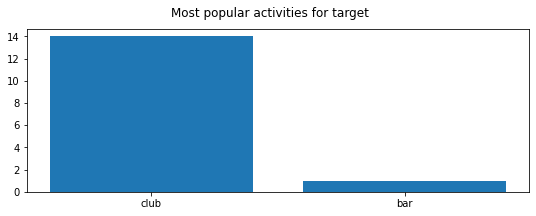
\includegraphics[scale=0.45]{target_activities}
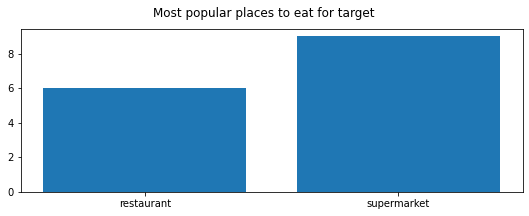
\includegraphics[scale=0.45]{target_places_to_eat}
	 
	Although we haven't computed it for this evaluation, we could think of a lot of other types of attacks, such as grouping different users by types of POIs to collect even more data and identify common habits between users.
	 
\subsection{Defenses}

	The main privacy risk with this app results from the fact that the user's locations are way too precise. We could add noise to the result in a way to obfuscate the real user's location, but there is an even simpler method. As we know, all POIs are distributed into cells. What we can do is, instead of using the user's real location to get the nearby POIs, we return all POIs in the same cell as the user. This way, the only thing an adversary could know from a user would be the cell he was in at the time of the query, which doesn't give much information on whether he was at home, at work, in a bar etc.
Since we converted the latitude longitude attributes to the cell id using the location to cell id method, there are no more unique locations, making it impossible for the adversary to determine the user's exact location (let's remind us that the grid cell is the size of a few kilometers square). Hence, the privacy of the user's location is respected. The trade-off is relatively small, as user will still be able to get the POIs he's interested in near his location, although some will be more far.
As we can see in the following graph, if the adversary tries to determine where the user spends most of his time, it is hard to tell.

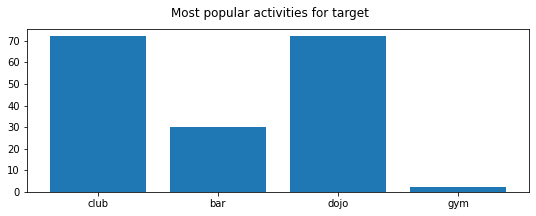
\includegraphics[scale=0.5]{target_activities_defense}

The problem is that it doesn't increase drastically the privacy, as for instance a cell containing only one type of POI could still let the adversary infer some information on the user's habit. 
What we could do is add dummy values to the POIs, although this would greatly reduce the utility of the app. We could also add noise to the timestamp so that an adversary can't determine the exact time the user was at some place.
	 
\section{Cell Fingerprinting via Network Traffic Analysis}
\subsection{Implementation details}
Data Collection : We used a shell script \emph{capture.sh} that we implemented in order to collect the data. Our shell script works as follow : we made 6 iteration where we queried  every grid\textunderscore id for every query . Thus we made a total of 600 queries to collect the data to build our ML model. We used the command tcpdump in order to obtain the packet captures for each query and write each corresponding .pcap file in the directory called pcaps . We used port 9050 to connect as this is known to be a port used for Tor connection . The data we give to the classifier are the bytes of each packets header for which the length is 66 as we saw that this was the most redundant length for the header. For each corresponding query of grid\textunderscore id we limit our-self to take the first 250 packets for which the header length is 66 , i.e our feature vector is at most 66x250 = 13200 bits .  

\subsection{Evaluation}
We used a Random Forest Classifier in order to predict the grid\textunderscore id when making a query. To evaluate our classifier with the data collected we performed a 5-fold cross validation . The metrics for the performance was a tuple containing : the accuracy\textunderscore score which we obtained a value of : 0.15 so 15 \% , the mean\textunderscore squared \textunderscore error which we obtained a value of 1254 and the explained\textunderscore variance \textunderscore score which we obtained a value of : -0.43 . For the explained\textunderscore variance \textunderscore score the best possible score is 1.0, lower values are worse.

\subsection{Discussion and Countermeasures}
Unfortunately we didn't have enough time to collect more data as this is quite a small data set for Machine Learning, making our classifier performing quite poorly . With more time and more parameters tuning we are confident that that we could get way better results and that the attack could be quite successful . 
As this is a Machine Learning powerful attack it can be hard to countermeasure this attack . One possible countermeasure could be that the server returns packets of length 66 with noise information that wouldn't alter the result of the user's query . Another countermeasure could be to make all the packets of the same random size every time for each query . Like than the attacker could not use the size of packets as potential information to infer the grid\textunderscore id .

\bibliographystyle{IEEEtran}
\bibliography{bib}
\end{document}

\bibliographystyle{IEEEtran}
\bibliography{bib}
\end{document}
